% Provenance (never printed): cycle 3 "La planete Terre" (the shaping of
% landscapes: erosion, transport and deposition by running water; rivers
% from source to mouth; floods); see sources/book1/PROVENANCE.md.
% Book 1, grade 5, chapter 1.
\chapter{Air Membentuk Daratan}\label{ch:g5:water-shapes-the-land}

Sepanjang malam, badai menderu di atap sekolah. Pagi harinya langit mulai
cerah, dan Lena serta Tom berlari ke \omterm{def:g1:landscapes-around-us:water}{sungai} kecil di belakang taman bermain.
Kemarin airnya jernih dan tenang: mereka bisa menghitung \omterm{def:g3:stones-pebbles-sand:pebble}{kerakal} di
dasarnya. Hari ini \omterm{def:g1:landscapes-around-us:water}{sungai} itu lebar, deras, dan cokelat, seperti warna
cokelat susu. \omterm{def:g1:landscapes-around-us:water}{Sungai} itu membawa ranting, daun, dan sesuatu yang tidak bisa
mereka lihat satu per satu: \omterm{def:g3:stones-pebbles-sand:sand}{lumpur} dan \omterm{def:g3:stones-pebbles-sand:sand}{pasir}, yang terkikis dari tepinya dan
dari ladang-ladang di hulu.

``Ke mana semua \omterm{def:g3:stones-pebbles-sand:sand}{lumpur} itu pergi?'' tanya Tom. Ke hilir, sedikit lebih jauh
setiap menit. \omterm{def:g1:landscapes-around-us:water}{Sungai} kecil itu sedang mengangkut daratan, butir demi butir.
Dalam bab ini kita mengikuti butir-butir itu, dari \omterm{def:g3:stones-pebbles-sand:rock}{batuan} asalnya sampai ke
tempat mereka mengendap.

\begin{omfigure}
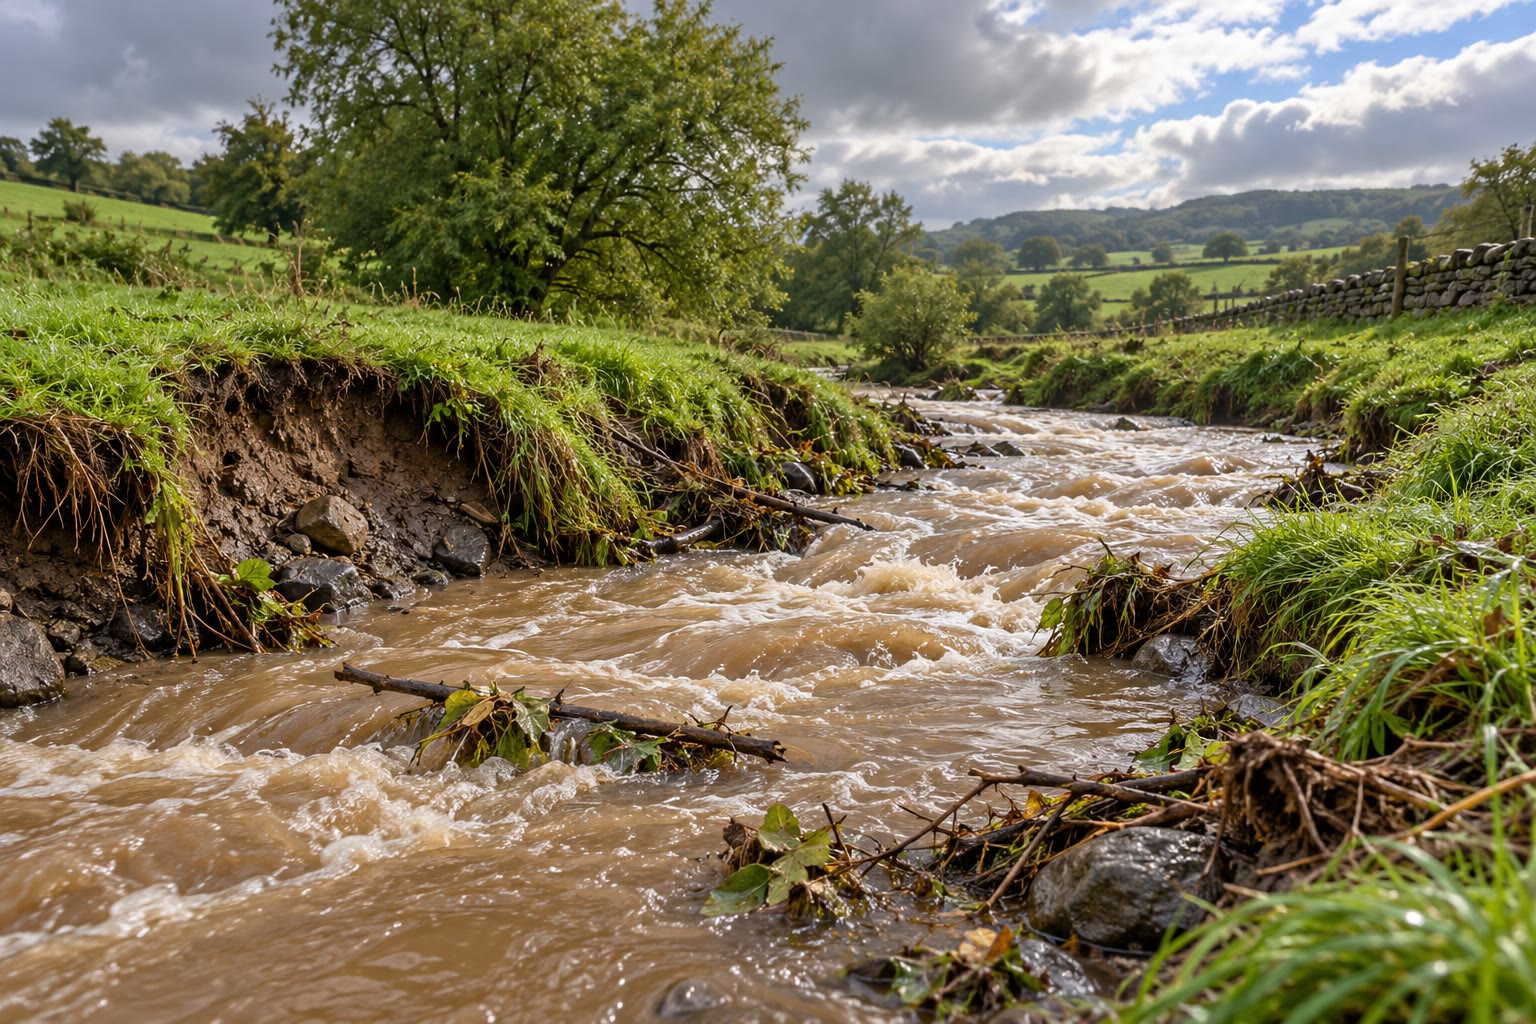
\includegraphics[width=0.5\linewidth]{images/book1/ai/g5-brown-stream.jpg}

{\small Sebuah \omterm{def:g1:landscapes-around-us:water}{sungai} kecil pada pagi hari setelah badai: airnya cokelat oleh
\omterm{def:g3:stones-pebbles-sand:sand}{lumpur} dan \omterm{def:g3:stones-pebbles-sand:sand}{pasir} yang dibawanya.}
\end{omfigure}

\begin{recall}
\omterm{def:g3:stones-pebbles-sand:rock}{Batuan} adalah bahan keras penyusun Bumi; jika pecah menjadi kepingan, \omterm{def:g3:stones-pebbles-sand:rock}{batuan}
menghasilkan batu, \omterm{def:g3:stones-pebbles-sand:pebble}{kerakal} yang dibulatkan oleh air, \omterm{def:g3:stones-pebbles-sand:sand}{pasir} yang butirnya
dapat kita lihat satu per satu, dan \omterm{def:g3:stones-pebbles-sand:sand}{lumpur} yang butirnya terlalu kecil untuk
dilihat (\cref{ch:g3:stones-pebbles-sand}). \omterm{def:g1:landscapes-around-us:water}{Sungai} mengalir terus-menerus di
dalam alur yang panjang, dari daratan yang lebih tinggi turun ke \omterm{def:g1:landscapes-around-us:water}{danau} atau
ke \omterm{def:g2:water-on-earth:ocean}{laut} (\cref{ch:g1:landscapes-around-us}). \omterm{def:g4:clouds-rain-snow:precipitation}{Hujan} yang jatuh di daratan
mengalir ke \omterm{def:g1:landscapes-around-us:water}{sungai-sungai} kecil dan \omterm{def:g1:landscapes-around-us:water}{sungai}, yang membawa air kembali ke \omterm{def:g2:water-on-earth:ocean}{laut}
(\cref{ch:g2:water-on-earth}).
\end{recall}

\section{Batuan pecah di tempatnya}

\omterm{def:g3:stones-pebbles-sand:rock}{Batuan} yang paling keras pun tidak bertahan selamanya. Di tempat yang
terbuka, di bawah matahari, \omterm{def:g4:clouds-rain-snow:precipitation}{hujan}, dan embun beku, \omterm{def:g3:stones-pebbles-sand:rock}{batuan} itu perlahan-lahan
retak dan hancur.

\begin{definition}[Pelapukan]\label{def:g5:water-shapes-the-land:weathering}
Yang disebut \emph{pelapukan}\index{pelapukan} adalah hancurnya \omterm{def:g3:stones-pebbles-sand:rock}{batuan} secara
perlahan di tempatnya, oleh embun beku, oleh air, oleh akar tumbuhan, dan
oleh panas dan dingin. \omterm{def:g3:stones-pebbles-sand:rock}{Batuan} pecah menjadi kepingan, tetapi kepingannya
tetap di tempat.
\end{definition}

Embun beku adalah salah satu alat \omterm{def:g5:water-shapes-the-land:weathering}{pelapukan} yang paling kuat. Air \omterm{def:g4:clouds-rain-snow:precipitation}{hujan}
meresap ke dalam retakan tipis pada \omterm{def:g3:stones-pebbles-sand:rock}{batuan}. Pada malam yang dingin, air itu
membeku, dan ketika air membeku, volumenya bertambah sedikit: es menekan
dinding retakan dan membukanya sedikit lebih lebar. Keesokan harinya es itu
mencair, lebih banyak air meresap masuk, dan pada malam berikutnya air itu
membeku lagi. Setelah banyak musim dingin, sekeping \omterm{def:g3:stones-pebbles-sand:rock}{batuan} terlepas.

\begin{omfigure}
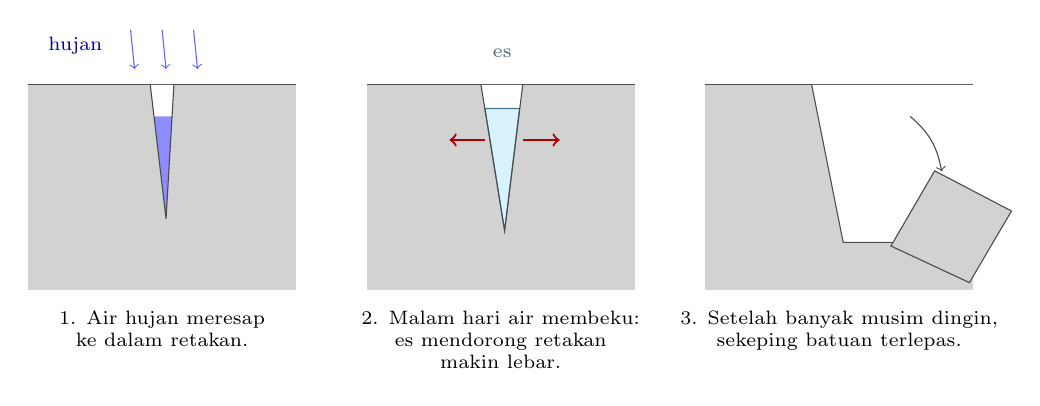
\begin{tikzpicture}[x=1cm, y=1cm, font=\scriptsize]
  \foreach \i/\t in {0/{1. Air hujan meresap\\ke dalam retakan.},
                     4.3/{2. Malam hari air membeku:\\es mendorong retakan\\makin lebar.},
                     8.6/{3. Setelah banyak musim dingin,\\sekeping batuan terlepas.}} {
    \begin{scope}[xshift=\i cm]
      \fill[gray!35] (0,0) rectangle (3.4,2.6);
      \draw[gray!60!black] (0,2.6) -- (3.4,2.6);
      \node[align=center, anchor=north] at (1.7,-0.15) {\t};
    \end{scope}
  }
  % panel 1: thin crack with water
  \fill[white] (1.55,2.6) -- (1.75,0.9) -- (1.85,2.6) -- cycle;
  \fill[blue!45] (1.6,2.2) -- (1.75,0.9) -- (1.83,2.2) -- cycle;
  \draw[gray!60!black] (1.55,2.6) -- (1.75,0.9) -- (1.85,2.6);
  \foreach \x in {1.3,1.7,2.1} \draw[blue!60, ->] (\x,3.3) -- (\x+0.05,2.8);
  \node[blue!60!black] at (0.6,3.1) {hujan};
  % panel 2: wider crack with ice
  \begin{scope}[xshift=4.3cm]
    \fill[white] (1.45,2.6) -- (1.75,0.75) -- (1.98,2.6) -- cycle;
    \fill[cyan!15] (1.5,2.3) -- (1.75,0.75) -- (1.94,2.3) -- cycle;
    \draw[cyan!50!black] (1.5,2.3) -- (1.75,0.75) -- (1.94,2.3) -- cycle;
    \draw[gray!60!black] (1.45,2.6) -- (1.75,0.75) -- (1.98,2.6);
    \draw[red!70!black, thick, <-] (1.05,1.9) -- (1.5,1.9);
    \draw[red!70!black, thick, ->] (1.98,1.9) -- (2.45,1.9);
    \node[cyan!40!black] at (1.72,3.0) {es};
  \end{scope}
  % panel 3: broken block
  \begin{scope}[xshift=8.6cm]
    \fill[white] (1.35,2.6) -- (1.75,0.6) -- (3.4,0.6) -- (3.4,2.6) -- cycle;
    \draw[gray!60!black] (1.35,2.6) -- (1.75,0.6) -- (3.4,0.6);
    \fill[gray!35, draw=gray!60!black, rotate around={-25:(2.9,0.3)}]
      (2.3,0.3) -- (2.4,1.4) -- (3.5,1.35) -- (3.4,0.3) -- cycle;
    \draw[gray!60!black, ->] (2.6,2.2) to[bend left=20] (3.0,1.5);
  \end{scope}
\end{tikzpicture}

{\small Embun beku memecahkan \omterm{def:g3:stones-pebbles-sand:rock}{batuan}. Setiap malam yang membeku, es di dalam
retakan mendorong sedikit; setelah banyak musim dingin, retakan itu cukup
lebar sehingga sekeping \omterm{def:g3:stones-pebbles-sand:rock}{batuan} terlepas.}
\end{omfigure}

Di bawah tebing \omterm{def:g3:stones-pebbles-sand:rock}{batuan} gundul yang tinggi di \omterm{def:g4:world-physical-map:range}{pegunungan}, kepingan yang
dipecahkan oleh embun beku meluncur dan berguling ke bawah, lalu menumpuk
menjadi lereng batu-batu tajam. Batu-batu itu tidak bulat: belum ada air
yang menggulingkannya.

\begin{omfigure}
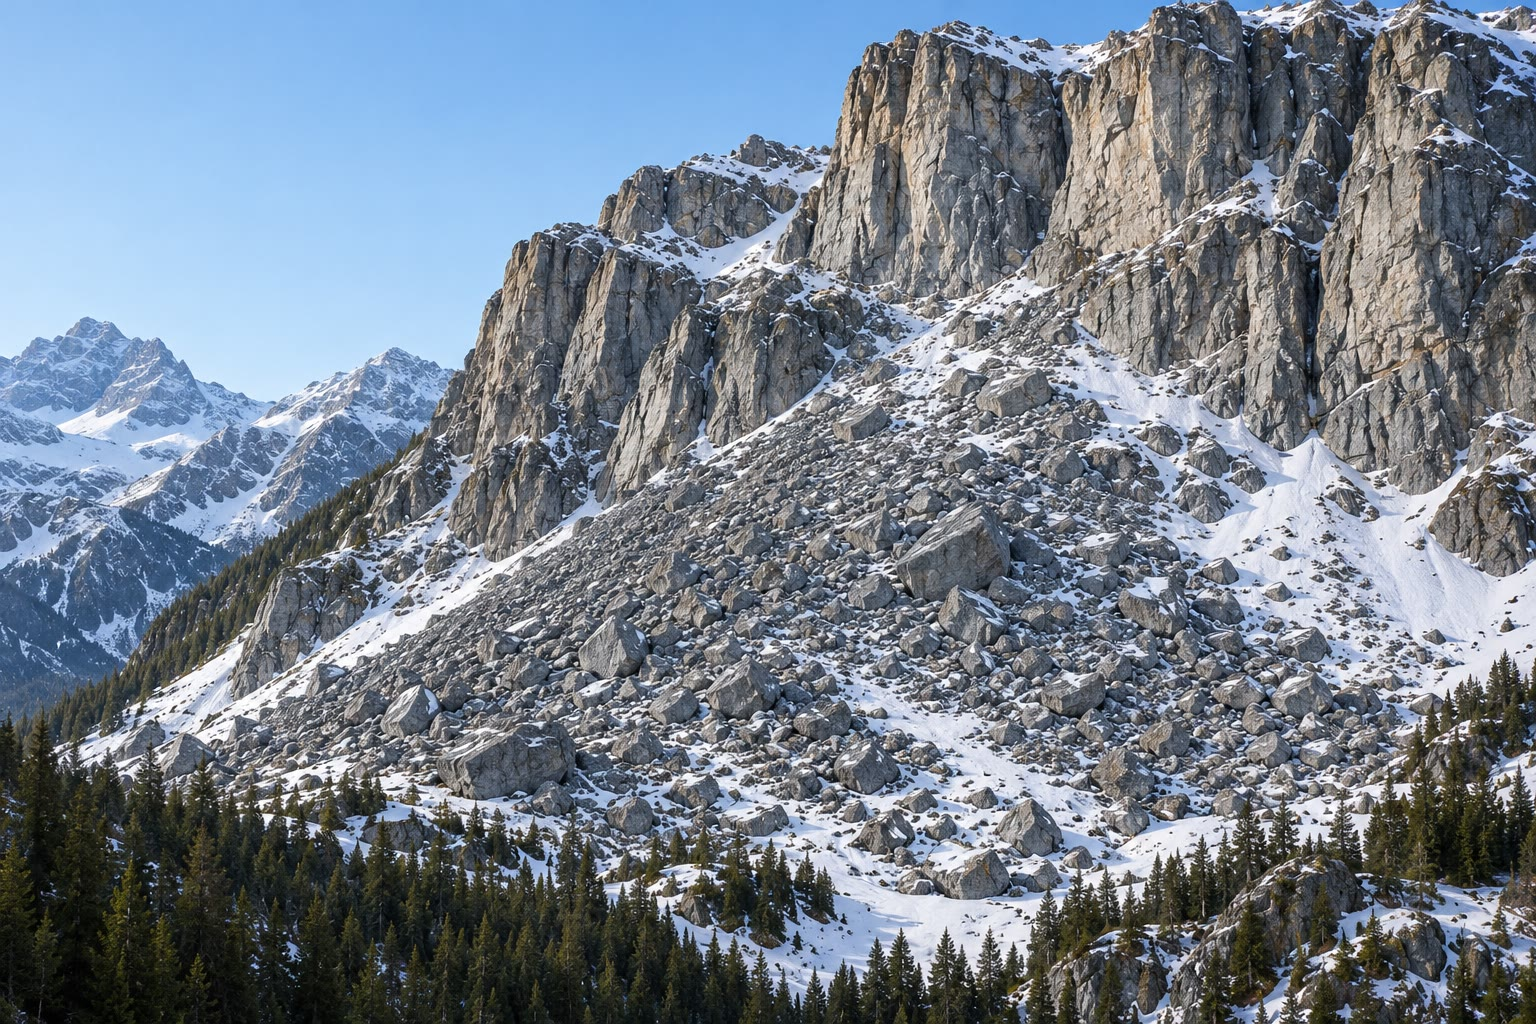
\includegraphics[width=0.5\linewidth]{images/book1/ai/g5-frost-scree.jpg}

{\small Di bawah tebing \omterm{def:g1:landscapes-around-us:landform}{gunung}, lereng batu-batu bersudut tajam yang
dipecahkan oleh embun beku, dilihat dari seberang \omterm{def:g1:landscapes-around-us:landform}{lembah}.}
\end{omfigure}

Tumbuhan juga ikut membantu. Akar pohon menyusup ke dalam retakan dan, ketika
akar itu makin tebal dari tahun ke tahun, akar itu membelah \omterm{def:g3:stones-pebbles-sand:rock}{batuan} seperti
baji yang bekerja perlahan. Air \omterm{def:g4:clouds-rain-snow:precipitation}{hujan} sendiri perlahan-lahan melunakkan
sebagian \omterm{def:g3:stones-pebbles-sand:rock}{batuan} dan mengubahnya menjadi tanah liat dan \omterm{def:g3:stones-pebbles-sand:sand}{pasir}: begitulah
tanah mendapat butir-butir mineralnya.

\section{Air mengangkut kepingan-kepingan itu}

Begitu \omterm{def:g3:stones-pebbles-sand:rock}{batuan} pecah, kepingannya dapat berpindah. Harus ada sesuatu yang
mengangkutnya.

\begin{definition}[Erosi]\label{def:g5:water-shapes-the-land:erosion}
Yang disebut \emph{erosi}\index{erosi} adalah terkikisnya daratan dan
terangkutnya kepingan \omterm{def:g3:stones-pebbles-sand:rock}{batuan}, terutama oleh air yang mengalir, tetapi juga
oleh angin, oleh es, dan oleh ombak \omterm{def:g2:water-on-earth:ocean}{laut}.
\end{definition}

Air yang mengalir melakukan sebagian besar pekerjaan itu. \omterm{def:g4:clouds-rain-snow:precipitation}{Hujan} menghanyutkan
tanah dan butiran menuruni lereng ke \omterm{def:g1:landscapes-around-us:water}{sungai-sungai} kecil; \omterm{def:g1:landscapes-around-us:water}{sungai-sungai} kecil
itu mengikis lebih banyak lagi dari tepinya sendiri, seperti \omterm{def:g1:landscapes-around-us:water}{sungai} kecil
Tom dan Lena setelah badai. Makin deras air mengalir, makin banyak yang
dapat diangkutnya, dan makin besar kepingan yang dapat dipindahkannya:
\omterm{def:g1:landscapes-around-us:water}{sungai} kecil yang tenang hanya membawa \omterm{def:g3:stones-pebbles-sand:sand}{lumpur} halus; \omterm{def:g1:landscapes-around-us:water}{sungai} kecil yang
sedang \omterm{def:g5:water-shapes-the-land:flood}{banjir} menggulingkan \omterm{def:g3:stones-pebbles-sand:pebble}{kerakal} dan bahkan bongkah di sepanjang
dasarnya.

Dalam perjalanannya, batu-batu itu saling berbenturan dan membentur dasar
\omterm{def:g1:landscapes-around-us:water}{sungai}. Sudut-sudutnya patah, dan batu-batu itu menjadi \omterm{def:g3:stones-pebbles-sand:pebble}{kerakal} yang bulat,
lalu butiran yang makin lama makin kecil: \omterm{def:g3:stones-pebbles-sand:sand}{pasir} dan \omterm{def:g3:stones-pebbles-sand:sand}{lumpur}.

Angin melakukan pekerjaan yang sama di tempat-tempat kering, tempat tidak
ada yang menahan \omterm{def:g3:stones-pebbles-sand:sand}{pasir}: angin meniupnya menjadi \omterm{def:g1:landscapes-around-us:landform}{bukit} \omterm{def:g3:stones-pebbles-sand:sand}{pasir}. Es, di
\omterm{def:g4:world-physical-map:range}{pegunungan} dan di dekat \omterm{def:g3:continents-and-oceans:poles}{kutub}, menyeret batu-batu di bawah bobotnya yang
sangat besar. Di \omterm{def:g1:landscapes-around-us:water}{pesisir}, ombak menghantam tebing dan menggulingkan \omterm{def:g3:stones-pebbles-sand:pebble}{kerakal}
di pantai maju dan mundur.

\begin{remark}[Berapa banyak?]\label{rem:g5:water-shapes-the-land:how-much}
Semua \omterm{def:g1:landscapes-around-us:water}{sungai} di dunia bersama-sama membawa lebih dari 12 miliar ton \omterm{def:g3:stones-pebbles-sand:sand}{lumpur}
dan \omterm{def:g3:stones-pebbles-sand:sand}{pasir} ke \omterm{def:g2:water-on-earth:ocean}{laut} setiap tahun. Itu kira-kira satu miliar ton setiap bulan.
% ledger: syvitski:modern-flux
\end{remark}

\section{Air meletakkan kepingan-kepingan itu}

\omterm{def:g1:landscapes-around-us:water}{Sungai} tidak dapat membawa muatannya selamanya. Di tempat alirannya
melambat, \omterm{def:g1:landscapes-around-us:water}{sungai} tidak lagi cukup kuat untuk memindahkan butiran yang
paling besar, dan butiran itu mengendap di dasarnya.

\begin{definition}[Pengendapan]\label{def:g5:water-shapes-the-land:deposition}
Yang disebut \emph{pengendapan}\index{pengendapan} adalah diletakkannya
kepingan \omterm{def:g3:stones-pebbles-sand:rock}{batuan} yang dibawa oleh air, angin, atau es, di tempat kepingan itu
melambat dan berhenti.
\end{definition}

Kepingan yang paling berat mengendap lebih dahulu: \omterm{def:g3:stones-pebbles-sand:pebble}{kerakal} jatuh di tempat
arus sedikit melemah, \omterm{def:g3:stones-pebbles-sand:sand}{pasir} di tempat arus makin melambat, dan \omterm{def:g3:stones-pebbles-sand:sand}{lumpur} halus
hanya di tempat airnya hampir diam, di \omterm{def:g1:landscapes-around-us:water}{danau} atau di \omterm{def:g2:water-on-earth:ocean}{laut}. Itulah sebabnya
dasar \omterm{def:g1:landscapes-around-us:water}{sungai} penuh \omterm{def:g3:stones-pebbles-sand:pebble}{kerakal} di \omterm{def:g4:world-physical-map:range}{pegunungan} dan berpasir atau berlumpur di
dekat \omterm{def:g2:water-on-earth:ocean}{laut}.

\omterm{def:g5:water-shapes-the-land:weathering}{Pelapukan}, \omterm{def:g5:water-shapes-the-land:erosion}{erosi}, dan \omterm{def:g5:water-shapes-the-land:deposition}{pengendapan} adalah tiga langkah dari satu perjalanan
panjang: \omterm{def:g3:stones-pebbles-sand:rock}{batuan} pecah di tempatnya, kepingannya diangkut, lalu diletakkan
di tempat lain. Perlahan-lahan air memindahkan \omterm{def:g1:landscapes-around-us:landform}{gunung}, butir demi butir,
turun ke \omterm{def:g1:landscapes-around-us:landform}{dataran} dan masuk ke \omterm{def:g2:water-on-earth:ocean}{laut}.

\begin{method}[Menamai apa yang dilakukan air]\label{met:g5:water-shapes-the-land:naming}
Untuk menamai apa yang terjadi pada \omterm{def:g3:stones-pebbles-sand:rock}{batuan} dalam sebuah gambar atau cerita,
ajukan tiga pertanyaan:
\begin{enumerate}
  \item Apakah \omterm{def:g3:stones-pebbles-sand:rock}{batuan} itu dipecahkan, tetapi kepingannya tetap di tempat?
        Itulah \emph{\omterm{def:g5:water-shapes-the-land:weathering}{pelapukan}}.
  \item Apakah kepingannya dikikis dan diangkut pergi? Itulah
        \emph{\omterm{def:g5:water-shapes-the-land:erosion}{erosi}}.
  \item Apakah kepingannya mengendap dan menumpuk? Itulah
        \emph{\omterm{def:g5:water-shapes-the-land:deposition}{pengendapan}}.
\end{enumerate}
\end{method}

\begin{example}[Sungai kecil setelah badai]\label{ex:g5:water-shapes-the-land:stream}
Air cokelat di \omterm{def:g1:landscapes-around-us:water}{sungai} kecil Tom dan Lena membawa \omterm{def:g3:stones-pebbles-sand:sand}{lumpur} yang terkikis dari
tepinya: itulah \omterm{def:g5:water-shapes-the-land:erosion}{erosi}. Seminggu kemudian, \omterm{def:g1:landscapes-around-us:water}{sungai} kecil itu jernih lagi, dan
selapis tipis \omterm{def:g3:stones-pebbles-sand:sand}{lumpur} menutupi dasar kolam yang tenang di ujung taman
bermain: itulah \omterm{def:g5:water-shapes-the-land:deposition}{pengendapan}.
\end{example}

\section{Sungai dari hulu sampai ke muara}

Setiap \omterm{def:g1:landscapes-around-us:water}{sungai} mempunyai awal dan akhir.

\begin{definition}[Hulu, muara, dan anak sungai]\label{def:g5:water-shapes-the-land:source-mouth}
Yang disebut \emph{hulu}\index{hulu (sungai)} sebuah \omterm{def:g1:landscapes-around-us:water}{sungai} adalah tempat
\omterm{def:g1:landscapes-around-us:water}{sungai} itu bermula: mata air, gletser yang mencair, atau daratan tinggi yang
basah tempat banyak aliran kecil bermula. \emph{Muara}\index{muara (sungai)}
\omterm{def:g1:landscapes-around-us:water}{sungai} adalah tempat \omterm{def:g1:landscapes-around-us:water}{sungai} itu berakhir, mengalir masuk ke \omterm{def:g2:water-on-earth:ocean}{laut}, \omterm{def:g1:landscapes-around-us:water}{danau},
atau \omterm{def:g1:landscapes-around-us:water}{sungai} yang lebih besar. Yang disebut
\emph{anak sungai}\index{anak sungai} adalah \omterm{def:g1:landscapes-around-us:water}{sungai} yang lebih kecil yang
mengalir masuk ke \omterm{def:g1:landscapes-around-us:water}{sungai} yang lebih besar.
\end{definition}

Sepanjang perjalanannya, sebuah \omterm{def:g1:landscapes-around-us:water}{sungai} berubah. Kita membagi panjangnya
menjadi tiga bagian: aliran \omterm{def:g5:water-shapes-the-land:source-mouth}{hulu}, aliran tengah, dan aliran hilir.

\begin{omfigure}
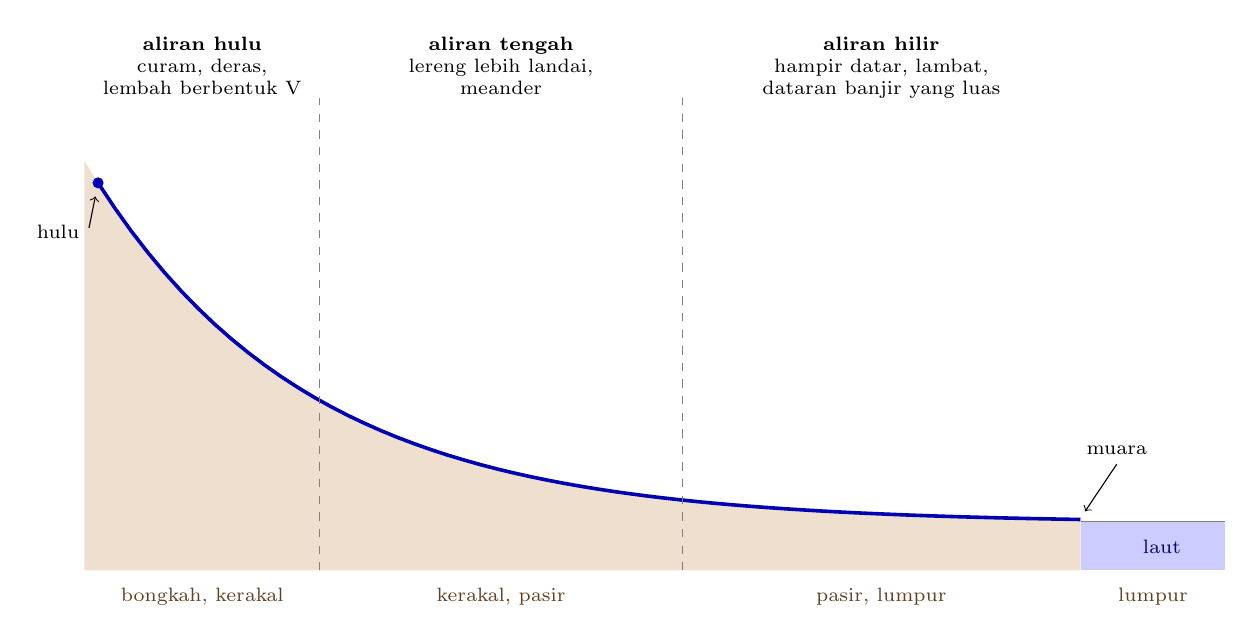
\begin{tikzpicture}[x=1.15cm, y=1cm, font=\scriptsize]
  % ground
  \fill[brown!25] (0,-0.6) -- plot[domain=0:11, samples=60]
    (\x,{4.6*exp(-\x/2.4)}) -- (11,-0.6) -- cycle;
  % sea
  \fill[blue!20] (11,-0.6) rectangle (12.6,0.02);
  \draw[blue!70!black, line width=1.3pt] plot[domain=0.15:11, samples=60]
    (\x,{4.6*exp(-\x/2.4)});
  \draw[gray] (11,0.02) -- (12.6,0.02);
  \node[blue!50!black] at (11.9,-0.3) {laut};
  % course limits
  \foreach \x in {2.6,6.6} \draw[gray, dashed] (\x,-0.6) -- (\x,5.4);
  \node[align=center, anchor=north] at (1.3,6.3) {\textbf{aliran hulu}\\curam, deras,\\lembah berbentuk V};
  \node[align=center, anchor=north] at (4.6,6.3) {\textbf{aliran tengah}\\lereng lebih landai,\\meander};
  \node[align=center, anchor=north] at (8.8,6.3) {\textbf{aliran hilir}\\hampir datar, lambat,\\dataran banjir yang luas};
  % source and mouth
  \fill[blue!70!black] (0.15,{4.6*exp(-0.15/2.4)}) circle (2pt);
  \node[anchor=east] at (0.05,3.7) {hulu};
  \draw[->] (0.05,3.75) -- (0.12,4.15);
  \node[anchor=south] at (11.4,0.75) {muara};
  \draw[->] (11.4,0.75) -- (11.05,0.15);
  % grain sizes
  \node[anchor=north, align=center, text=brown!50!black] at (1.3,-0.7) {bongkah, kerakal};
  \node[anchor=north, align=center, text=brown!50!black] at (4.6,-0.7) {kerakal, pasir};
  \node[anchor=north, align=center, text=brown!50!black] at (8.8,-0.7) {pasir, lumpur};
  \node[anchor=north, align=center, text=brown!50!black] at (11.8,-0.7) {lumpur};
\end{tikzpicture}

{\small Profil memanjang sebuah \omterm{def:g1:landscapes-around-us:water}{sungai}, dari \omterm{def:g5:water-shapes-the-land:source-mouth}{hulu} sampai ke muara (tingginya
sangat dibesar-besarkan). Di bawah: apa yang terdapat di dasarnya.}
\end{omfigure}

Pada \emph{aliran \omterm{def:g5:water-shapes-the-land:source-mouth}{hulu}}, di \omterm{def:g4:world-physical-map:range}{pegunungan}, \omterm{def:g1:landscapes-around-us:water}{sungai} masih muda dan curam. Airnya
menerjang turun, menggulingkan bongkah di sepanjang dasarnya, dan mengikis
\omterm{def:g3:stones-pebbles-sand:rock}{batuan} ke arah bawah. \omterm{def:g1:landscapes-around-us:water}{Sungai} itu menggali \omterm{def:g1:landscapes-around-us:landform}{lembah} sempit dengan dinding yang
curam, yang bentuknya seperti huruf V.

Pada \emph{aliran tengah}, lerengnya lebih landai. \omterm{def:g1:landscapes-around-us:water}{Sungai} berayun dari satu
sisi ke sisi lain dalam kelokan-kelokan besar.

\begin{definition}[Meander]\label{def:g5:water-shapes-the-land:meander}
Yang disebut \emph{meander}\index{meander} adalah kelokan \omterm{def:g1:landscapes-around-us:water}{sungai} yang
berliku-liku melintasi dasar \omterm{def:g1:landscapes-around-us:landform}{lembah} yang datar.
\end{definition}

\omterm{def:g5:water-shapes-the-land:meander}{Meander} tidak diam di tempat: \omterm{def:g5:water-shapes-the-land:meander}{meander} berpindah. Di sisi luar setiap
tikungan, air mengalir deras dan dalam: air itu menggerus tepi \omterm{def:g1:landscapes-around-us:water}{sungai},
yang lalu menjadi tebing kecil. Di sisi dalam tikungan, air mengalir
lambat: air itu menjatuhkan \omterm{def:g3:stones-pebbles-sand:sand}{pasir} dan \omterm{def:g3:stones-pebbles-sand:pebble}{kerikil}, yang membentuk pantai yang
landai. Dari tahun ke tahun, tepi luar terkikis mundur dan pantai di sisi
dalam bertambah, dan kelokan itu berayun makin lama makin lebar.

\begin{omfigure}
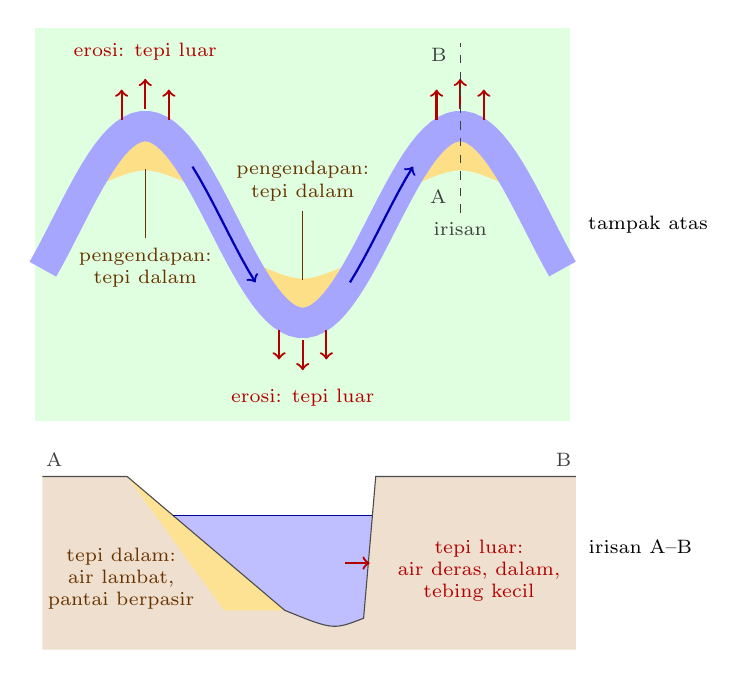
\begin{tikzpicture}[x=1cm, y=1cm, font=\scriptsize]
  % ---- map view ----
  \fill[green!12] (-0.4,-2.5) rectangle (6.4,2.5);
  % sand on the inner banks (drawn first, the river covers its edge)
  \foreach \c/\s in {1/1, 3/-1, 5/1}
    \fill[yellow!50!orange!45] (\c-0.6,\s*0.5) .. controls (\c,\s*1.5) ..
      (\c+0.6,\s*0.5) .. controls (\c,\s*0.75) .. cycle;
  % the river
  \draw[blue!35, line width=11pt] plot[domain=-0.3:6.3, samples=90]
    (\x,{1.25*sin(\x*90)});
  \draw[blue!70!black, ->, thick] plot[domain=1.6:2.4, samples=10]
    (\x,{1.25*sin(\x*90)});
  \draw[blue!70!black, ->, thick] plot[domain=3.6:4.4, samples=10]
    (\x,{1.25*sin(\x*90)});
  % erosion on the outer banks
  \foreach \c/\s in {1/1, 3/-1, 5/1}
    \foreach \d in {-0.3,0,0.3}
      \draw[red!70!black, thick, ->] (\c+\d,{\s*(1.25*cos(\d*90)+0.22)})
        -- (\c+\d,{\s*(1.25*cos(\d*90)+0.6)});
  \node[red!70!black] at (1,2.2) {erosi: tepi luar};
  \node[red!70!black] at (3,-2.2) {erosi: tepi luar};
  \node[orange!40!black, align=center] (d1) at (1,-0.55) {pengendapan:\\tepi dalam};
  \node[orange!40!black, align=center] (d2) at (3,0.55) {pengendapan:\\tepi dalam};
  \draw[orange!40!black] (d1.north) -- (1,0.7);
  \draw[orange!40!black] (d2.south) -- (3,-0.7);
  \draw[gray!50!black, dashed] (5,0.15) -- (5,2.3);
  \node[gray!50!black, anchor=north] at (5,0.15) {irisan};
  \node[gray!50!black, anchor=east] at (4.95,0.35) {A};
  \node[gray!50!black, anchor=east] at (4.95,2.15) {B};
  \node[anchor=west] at (6.5,0) {tampak atas};
  % ---- cut ----
  \begin{scope}[yshift=-4.1cm, xscale=0.77]
    \fill[brown!25] (-0.4,-1.3) -- (-0.4,0.9) -- (1,0.9) -- (3.6,-0.8)
      .. controls (4.4,-1.05) .. (4.9,-0.9) -- (5.1,0.9) -- (8.4,0.9)
      -- (8.4,-1.3) -- cycle;
    \fill[blue!25] (1.75,0.4) -- (3.6,-0.8) .. controls (4.4,-1.05) .. (4.9,-0.9)
      -- (5.04,0.4) -- cycle;
    \fill[yellow!50!orange!40] (1,0.9) -- (3.6,-0.8) -- (2.6,-0.8) -- cycle;
    \draw[gray!60!black] (-0.4,0.9) -- (1,0.9) -- (3.6,-0.8)
      .. controls (4.4,-1.05) .. (4.9,-0.9) -- (5.1,0.9) -- (8.4,0.9);
    \draw[blue!60!black] (1.75,0.4) -- (5.04,0.4);
    \node[orange!40!black, align=center] at (0.9,-0.4) {tepi dalam:\\air lambat,\\pantai berpasir};
    \node[red!70!black, align=center, anchor=west] at (5.3,-0.3) {tepi luar:\\air deras, dalam,\\tebing kecil};
    \draw[red!70!black, thick, ->] (4.6,-0.2) -- (5.0,-0.2);
    \node[gray!50!black, anchor=south] at (-0.2,0.9) {A};
    \node[gray!50!black, anchor=south] at (8.2,0.9) {B};
    \node[anchor=west] at (8.45,0) {irisan A--B};
  \end{scope}
\end{tikzpicture}

{\small Sebuah \omterm{def:g5:water-shapes-the-land:meander}{meander} dilihat dari atas, dan diiris melintang sepanjang garis
putus-putus A--B. Air menggerus tepi luar setiap tikungan dan menjatuhkan
\omterm{def:g3:stones-pebbles-sand:sand}{pasir} di tepi dalam: kelokan itu perlahan-lahan berpindah.}
\end{omfigure}

Kadang-kadang dua kelokan tumbuh begitu dekat sehingga, ketika \omterm{def:g5:water-shapes-the-land:flood}{banjir},
\omterm{def:g1:landscapes-around-us:water}{sungai} menerobos leher daratan yang sempit di antara keduanya dan mengambil
jalan pintas. Kelokan lama tertinggal sebagai \omterm{def:g1:landscapes-around-us:water}{danau} yang melengkung.

\begin{omfigure}
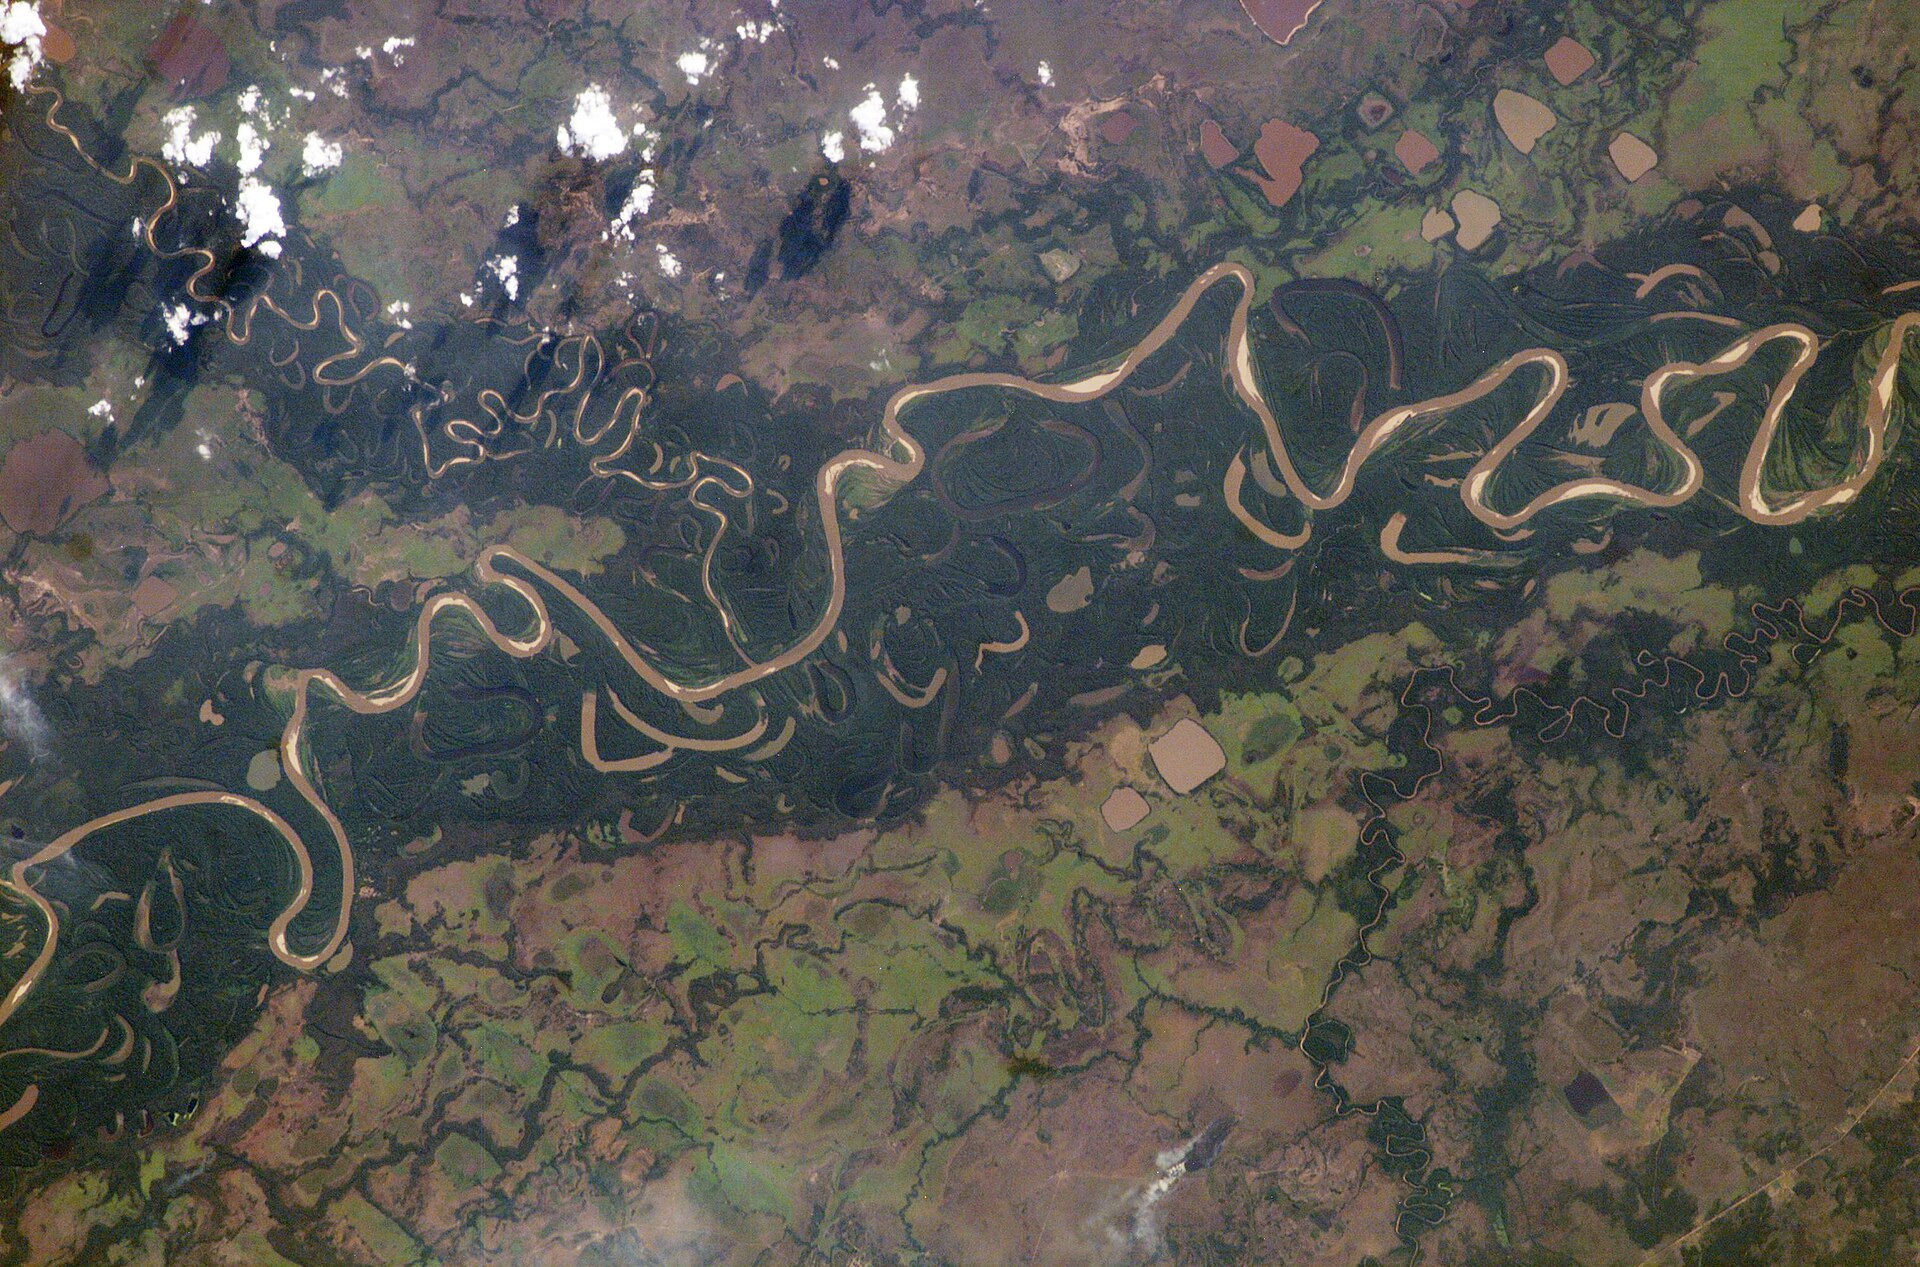
\includegraphics[width=0.52\linewidth]{images/book1/g5-mamore-meanders.jpg}

{\small \omterm{def:g1:landscapes-around-us:water}{Sungai} Mamoré, di dataran rendah Bolivia di Amerika Selatan, dilihat
dari Stasiun Antariksa Internasional. \omterm{def:g1:landscapes-around-us:water}{Sungai} yang cokelat itu berkelok-kelok
membentuk \omterm{def:g5:water-shapes-the-land:meander}{meander} di tengah hutan. Foto: NASA (domain publik).}\label{fig:g5:water-shapes-the-land:mamore}
% ledger: nasa:mamore-meanders
\end{omfigure}

Pada \emph{aliran hilir}, daratannya hampir datar. \omterm{def:g1:landscapes-around-us:water}{Sungai} mengalir lambat
melintasi dasar \omterm{def:g1:landscapes-around-us:landform}{lembah} yang lebar dan datar, yang tersusun dari \omterm{def:g3:stones-pebbles-sand:sand}{lumpur} dan
\omterm{def:g3:stones-pebbles-sand:sand}{pasir} yang diletakkannya sendiri selama waktu yang sangat lama.

\begin{omfigure}
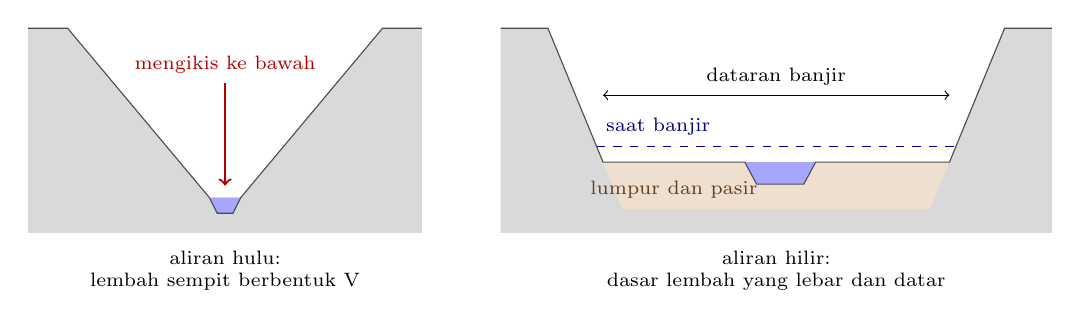
\begin{tikzpicture}[x=1cm, y=1cm, font=\scriptsize]
  % V-shaped valley
  \fill[gray!30] (0,0) -- (0,2.6) -- (0.5,2.6) -- (2.3,0.45) -- (2.7,0.45)
    -- (4.5,2.6) -- (5,2.6) -- (5,0) -- cycle;
  \fill[blue!35] (2.3,0.45) -- (2.4,0.25) -- (2.6,0.25) -- (2.7,0.45) -- cycle;
  \draw[gray!60!black] (0,2.6) -- (0.5,2.6) -- (2.3,0.45) -- (2.4,0.25)
    -- (2.6,0.25) -- (2.7,0.45) -- (4.5,2.6) -- (5,2.6);
  \draw[red!70!black, thick, ->] (2.5,1.9) -- (2.5,0.6);
  \node[red!70!black, anchor=south] at (2.5,1.9) {mengikis ke bawah};
  \node[align=center, anchor=north] at (2.5,-0.1) {aliran hulu:\\lembah sempit berbentuk V};
  % floodplain
  \begin{scope}[xshift=6cm]
    \fill[gray!30] (0,0) -- (0,2.6) -- (0.6,2.6) -- (1.3,0.9) -- (5.7,0.9)
      -- (6.4,2.6) -- (7,2.6) -- (7,0) -- cycle;
    \fill[brown!25] (1.3,0.9) -- (1.55,0.3) -- (5.45,0.3) -- (5.7,0.9) -- cycle;
    \fill[blue!35] (3.1,0.9) -- (3.25,0.62) -- (3.85,0.62) -- (4,0.9) -- cycle;
    \draw[gray!60!black] (0,2.6) -- (0.6,2.6) -- (1.3,0.9) -- (3.1,0.9)
      -- (3.25,0.62) -- (3.85,0.62) -- (4,0.9) -- (5.7,0.9) -- (6.4,2.6) -- (7,2.6);
    \draw[blue!60!black, dashed] (1.22,1.1) -- (5.78,1.1);
    \node[blue!50!black, anchor=south] at (2.0,1.12) {saat banjir};
    \node[brown!50!black] at (2.2,0.55) {lumpur dan pasir};
    \draw[<->] (1.3,1.75) -- (5.7,1.75);
    \node[anchor=south] at (3.5,1.75) {dataran banjir};
    \node[align=center, anchor=north] at (3.5,-0.1) {aliran hilir:\\dasar lembah yang lebar dan datar};
  \end{scope}
\end{tikzpicture}

{\small Penampang \omterm{def:g1:landscapes-around-us:landform}{lembah}, di \omterm{def:g4:world-physical-map:range}{pegunungan} dan di dekat \omterm{def:g2:water-on-earth:ocean}{laut} (skalanya tidak
sama). Saat \omterm{def:g5:water-shapes-the-land:flood}{banjir}, \omterm{def:g1:landscapes-around-us:water}{sungai} meluap ke seluruh \omterm{def:g5:water-shapes-the-land:flood}{dataran banjirnya}.}
\end{omfigure}

Akhirnya \omterm{def:g1:landscapes-around-us:water}{sungai} sampai di muaranya. Di sana airnya melambat hampir
sepenuhnya, dan \omterm{def:g1:landscapes-around-us:water}{sungai} menjatuhkan sisa muatannya. Di tempat ombak dan
pasang surut \omterm{def:g2:water-on-earth:ocean}{laut} terlalu lemah untuk menyapu semuanya, \omterm{def:g3:stones-pebbles-sand:sand}{lumpur} dan \omterm{def:g3:stones-pebbles-sand:sand}{pasir}
menumpuk, dan daratan baru tumbuh menjorok ke \omterm{def:g2:water-on-earth:ocean}{laut}.

\begin{definition}[Delta]\label{def:g5:water-shapes-the-land:delta}
Yang disebut \emph{delta}\index{delta} adalah daratan baru yang datar, yang
dibangun oleh \omterm{def:g1:landscapes-around-us:water}{sungai} di muaranya dari \omterm{def:g3:stones-pebbles-sand:sand}{lumpur} dan \omterm{def:g3:stones-pebbles-sand:sand}{pasir} yang diendapkannya.
\omterm{def:g1:landscapes-around-us:water}{Sungai} itu terbelah menjadi beberapa cabang yang menyebar di atasnya,
sering kali berbentuk seperti kipas.
\end{definition}

Namanya berasal dari huruf Yunani $\Delta$ (\omterm{def:g5:water-shapes-the-land:delta}{delta}), sebuah segitiga, karena
\omterm{def:g5:water-shapes-the-land:delta}{delta} \omterm{def:g1:landscapes-around-us:water}{Sungai} Nil, di Mesir, mempunyai bentuk seperti itu.

Ada \omterm{def:g1:landscapes-around-us:water}{sungai} yang berakhir tanpa \omterm{def:g5:water-shapes-the-land:delta}{delta}. Di tempat ombak dan pasang surut yang
kuat menyapu \omterm{def:g3:stones-pebbles-sand:sand}{lumpur}, \omterm{def:g1:landscapes-around-us:water}{sungai} berakhir pada muara yang lebar dan berbentuk
corong, tempat air \omterm{def:g2:water-on-earth:ocean}{laut} masuk dan keluar mengikuti pasang surut: sebuah
\emph{estuari}.

\begin{omfigure}
\begin{minipage}[b]{0.55\linewidth}\centering
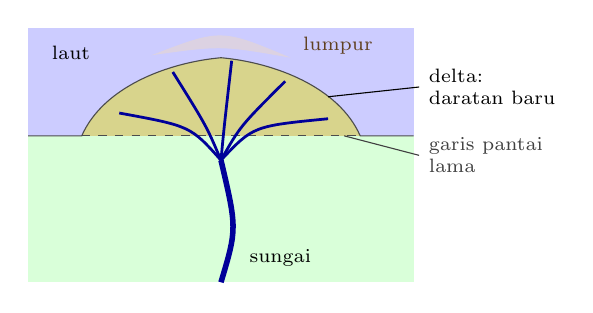
\begin{tikzpicture}[x=0.68cm, y=0.62cm, font=\scriptsize]
  \fill[blue!20] (-3.6,1.4) rectangle (3.6,3.6);
  \fill[green!15] (-3.6,-1.6) rectangle (3.6,1.4);
  % delta
  \fill[olive!35] (-2.6,1.4) .. controls (-2.2,2.4) and (-1,2.9)
    .. (0,3.0) .. controls (1,2.9) and (2.2,2.4) .. (2.6,1.4) -- cycle;
  \draw[gray!60!black] (-3.6,1.4) -- (-2.6,1.4) .. controls (-2.2,2.4) and
    (-1,2.9) .. (0,3.0) .. controls (1,2.9) and (2.2,2.4) .. (2.6,1.4) -- (3.6,1.4);
  \draw[gray!60!black, dashed] (-2.6,1.4) -- (2.6,1.4);
  % river and branches
  \draw[blue!60!black, line width=2pt] (0,-1.6) .. controls (0.3,-0.5) .. (0,0.9);
  \foreach \e in {-1.9,-0.9,0.2,1.2,2.0}
    \draw[blue!60!black, line width=1pt] (0,0.9) .. controls (\e*0.3,1.6) ..
      (\e,{2.95-0.3*\e*\e});
  % mud plume
  \fill[brown!30, opacity=0.5] (-1.3,3.05) .. controls (0,3.6) .. (1.3,3.0)
    .. controls (0,3.25) .. cycle;
  \node[align=center] at (-2.8,3.1) {laut};
  \node[anchor=west, brown!50!black] at (1.35,3.25) {lumpur};
  \node[anchor=west, align=left] at (3.7,2.4) {delta:\\daratan baru};
  \draw (3.7,2.4) -- (2.0,2.2);
  \node[anchor=west, align=left, gray!50!black] at (3.7,1.0) {garis pantai\\lama};
  \draw[gray!50!black] (3.7,1.0) -- (2.3,1.4);
  \node[anchor=west] at (0.35,-1.1) {sungai};
\end{tikzpicture}
\end{minipage}\hfill
\begin{minipage}[b]{0.3\linewidth}\centering
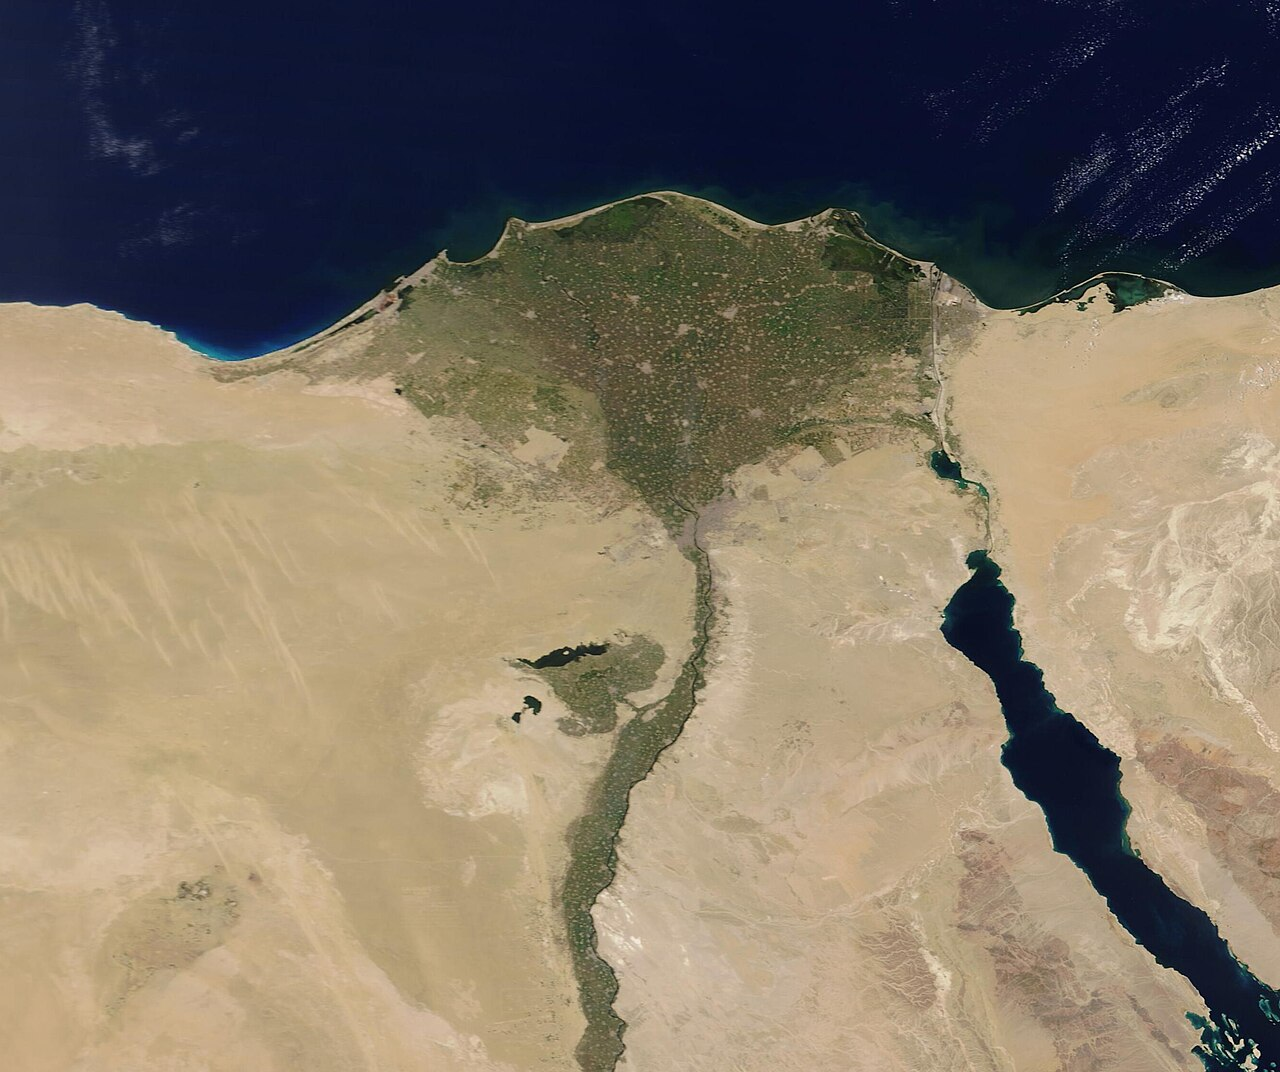
\includegraphics[width=\linewidth]{images/book1/g5-nile-delta-modis.jpg}
\end{minipage}

{\small Kiri: sebuah \omterm{def:g5:water-shapes-the-land:delta}{delta} dilihat dari atas; \omterm{def:g3:stones-pebbles-sand:sand}{lumpur} dan \omterm{def:g3:stones-pebbles-sand:sand}{pasir} yang
diendapkan oleh cabang-cabang \omterm{def:g1:landscapes-around-us:water}{sungai} membangun daratan baru melewati garis
pantai lama. Kanan: \omterm{def:g5:water-shapes-the-land:delta}{delta} \omterm{def:g1:landscapes-around-us:water}{Sungai} Nil, di Mesir, dari satelit (\omterm{def:g2:water-on-earth:ocean}{laut} di
bagian atas): kipas hijau berupa ladang di atas \omterm{def:g3:stones-pebbles-sand:sand}{lumpur} \omterm{def:g1:landscapes-around-us:water}{sungai}, di tengah
gurun. Foto: NASA (domain publik).}
% ledger: nasa:nile-delta-modis
\end{omfigure}

\section{Banjir}

Setelah berhari-hari \omterm{def:g4:clouds-rain-snow:precipitation}{hujan}, atau ketika \omterm{def:g4:clouds-rain-snow:precipitation}{salju} mencair dengan cepat pada
musim semi, sebuah \omterm{def:g1:landscapes-around-us:water}{sungai} menerima lebih banyak air daripada yang dapat
ditampung alurnya.

\begin{definition}[Banjir dan dataran banjir]\label{def:g5:water-shapes-the-land:flood}
Yang disebut \emph{banjir}\index{banjir} terjadi ketika air menggenangi
daratan yang biasanya kering. \omterm{def:g1:landscapes-around-us:water}{Sungai} banjir ketika airnya naik melewati
tepinya dan meluap ke daratan datar di kedua sisinya. Daratan datar itu,
yang dari waktu ke waktu digenangi \omterm{def:g1:landscapes-around-us:water}{sungai}, adalah
\emph{dataran banjir}\index{dataran banjir} \omterm{def:g1:landscapes-around-us:water}{sungai} itu.
\end{definition}

\begin{omfigure}
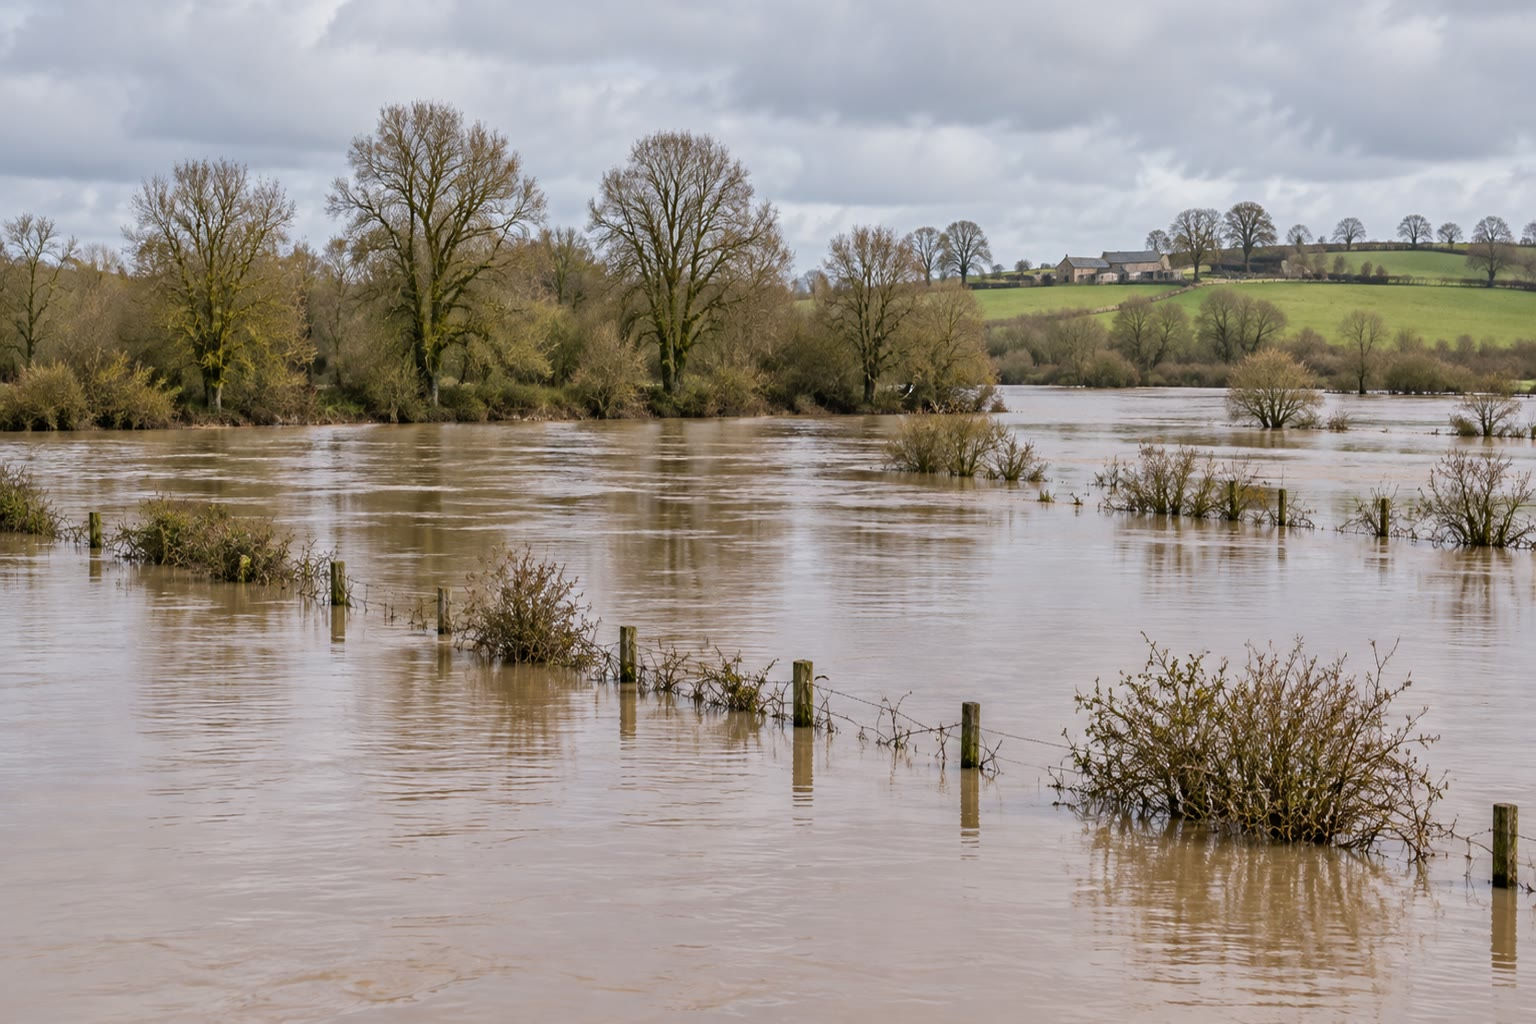
\includegraphics[width=0.5\linewidth]{images/book1/ai/g5-flooded-meadow.jpg}

{\small Padang rumput yang tergenang air \omterm{def:g5:water-shapes-the-land:flood}{banjir} setelah berhari-hari \omterm{def:g4:clouds-rain-snow:precipitation}{hujan}.
Deretan pohon menandai tepi \omterm{def:g1:landscapes-around-us:water}{sungai} yang biasa; rumah pertanian berdiri di
tanah yang lebih tinggi.}
\end{omfigure}

\omterm{def:g1:landscapes-around-us:water}{Sungai} yang \omterm{def:g5:water-shapes-the-land:flood}{banjir} tidak sedang melakukan sesuatu yang aneh: \omterm{def:g1:landscapes-around-us:water}{sungai} itu
melakukan apa yang selalu dilakukan \omterm{def:g1:landscapes-around-us:water}{sungai}. \omterm{def:g5:water-shapes-the-land:flood}{Dataran banjir} adalah
wilayahnya. Sebenarnya \omterm{def:g1:landscapes-around-us:water}{sungai} itulah yang membangunnya: setiap \omterm{def:g5:water-shapes-the-land:flood}{banjir}
meninggalkan selapis tipis \omterm{def:g3:stones-pebbles-sand:sand}{lumpur} di ladang, dan itulah sebabnya \omterm{def:g5:water-shapes-the-land:flood}{dataran
banjir} mempunyai tanah yang begitu subur. Dahulu kala, para petani di
Mesir menunggu \omterm{def:g5:water-shapes-the-land:flood}{banjir} tahunan \omterm{def:g1:landscapes-around-us:water}{Sungai} Nil, yang mengairi ladang mereka dan
membawakan \omterm{def:g3:stones-pebbles-sand:sand}{lumpur} baru.

Akan tetapi, \omterm{def:g5:water-shapes-the-land:flood}{banjir} berbahaya bagi orang yang tinggal di \omterm{def:g5:water-shapes-the-land:flood}{dataran banjir}.
Rumah yang dibangun di atasnya bisa terisi air, dan air \omterm{def:g5:water-shapes-the-land:flood}{banjir} yang deras
bisa menghanyutkan mobil dan manusia. Kota yang bijak membangun di tanah
yang lebih tinggi dan membiarkan \omterm{def:g5:water-shapes-the-land:flood}{dataran banjir} untuk ladang, padang
rumput, dan taman. Dalam \cref{ch:g5:natural-hazards} kita akan melihat
bagaimana orang bersiap menghadapi \omterm{def:g5:water-shapes-the-land:flood}{banjir} dan tetap selamat.

\begin{safety}
Jangan pernah berjalan, bersepeda, atau bermain di air \omterm{def:g5:water-shapes-the-land:flood}{banjir}, dan jangan
pernah mendekati \omterm{def:g1:landscapes-around-us:water}{sungai} yang sedang \omterm{def:g5:water-shapes-the-land:flood}{banjir}: airnya lebih kuat dan lebih
dalam daripada kelihatannya, dan air itu bisa menyembunyikan lubang dan
saluran air yang terbuka. Jauhilah tempat itu sampai orang dewasa yang
bertanggung jawab mengatakan bahwa keadaan sudah aman.
\end{safety}

\section{Latihan}

\begin{exercise}[$\star$]\label{exo:g5:water-shapes-the-land:1}
Namai prosesnya: \omterm{def:g5:water-shapes-the-land:weathering}{pelapukan}, \omterm{def:g5:water-shapes-the-land:erosion}{erosi}, atau \omterm{def:g5:water-shapes-the-land:deposition}{pengendapan}?
\begin{enumerate}
  \item[(a)] Es di dalam retakan membelah sebuah \omterm{def:g3:stones-pebbles-sand:rock}{batuan} di \omterm{def:g1:landscapes-around-us:landform}{gunung}.
  \item[(b)] \omterm{def:g1:landscapes-around-us:water}{Sungai} yang sedang \omterm{def:g5:water-shapes-the-land:flood}{banjir} mengangkut \omterm{def:g3:stones-pebbles-sand:sand}{pasir} dari tepinya.
  \item[(c)] Selapis \omterm{def:g3:stones-pebbles-sand:sand}{lumpur} mengendap di dasar \omterm{def:g1:landscapes-around-us:water}{danau} yang tenang.
  \item[(d)] Akar pohon membelah tembok batu.
\end{enumerate}
\end{exercise}

\begin{exercise}[$\star$]\label{exo:g5:water-shapes-the-land:2}
Apa yang dimaksud dengan \omterm{def:g5:water-shapes-the-land:source-mouth}{hulu} \omterm{def:g1:landscapes-around-us:water}{sungai}? Apa muaranya? Apa \omterm{def:g5:water-shapes-the-land:source-mouth}{anak sungai}?
\end{exercise}

\begin{exercise}[$\star$]\label{exo:g5:water-shapes-the-land:3}
Urutkan bagian-bagian \omterm{def:g1:landscapes-around-us:water}{sungai} berikut, dari \omterm{def:g5:water-shapes-the-land:source-mouth}{hulu} sampai ke \omterm{def:g2:water-on-earth:ocean}{laut}: \omterm{def:g5:water-shapes-the-land:meander}{meander};
\omterm{def:g5:water-shapes-the-land:delta}{delta}; \omterm{def:g1:landscapes-around-us:landform}{lembah} sempit berbentuk V; \omterm{def:g5:water-shapes-the-land:source-mouth}{hulu}.
\end{exercise}

\begin{exercise}[$\star$]\label{exo:g5:water-shapes-the-land:4}
Benar atau salah? Jelaskan.
\begin{enumerate}
  \item[(a)] \omterm{def:g3:stones-pebbles-sand:rock}{Batuan} keras tidak pernah berubah.
  \item[(b)] \omterm{def:g1:landscapes-around-us:water}{Sungai} yang deras dapat membawa batu yang lebih besar daripada \omterm{def:g1:landscapes-around-us:water}{sungai} yang lambat.
  \item[(c)] \omterm{def:g3:stones-pebbles-sand:sand}{Lumpur} yang paling halus mengendap lebih dahulu, di dekat \omterm{def:g5:water-shapes-the-land:source-mouth}{hulu}.
\end{enumerate}
\end{exercise}

\begin{exercise}[$\star$]\label{exo:g5:water-shapes-the-land:5}
Berikut ini sebuah tikungan \omterm{def:g1:landscapes-around-us:water}{sungai} dilihat dari atas.

\begin{center}
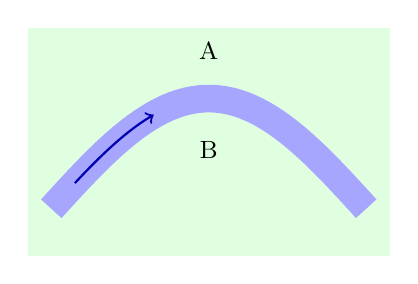
\begin{tikzpicture}[x=1cm, y=1cm, font=\small]
  \fill[green!12] (-0.3,-0.6) rectangle (4.3,2.3);
  \draw[blue!35, line width=10pt] plot[domain=0:4, samples=50]
    (\x,{1.4*sin(\x*45)});
  \draw[blue!70!black, ->, thick] plot[domain=0.3:1.3, samples=20]
    (\x,{1.4*sin(\x*45)});
  \node at (2,2.0) {A};
  \node at (2,0.75) {B};
\end{tikzpicture}
\end{center}
Di tepi manakah, A atau B, \omterm{def:g1:landscapes-around-us:water}{sungai} menggerus daratan? Di tepi manakah \omterm{def:g1:landscapes-around-us:water}{sungai}
menjatuhkan \omterm{def:g3:stones-pebbles-sand:sand}{pasir}?
\end{exercise}

\begin{exercise}[$\star$]\label{exo:g5:water-shapes-the-land:6}
Di \omterm{def:g4:world-physical-map:range}{pegunungan}, dasar \omterm{def:g1:landscapes-around-us:water}{sungai} tertutup batu-batu besar. Di dekat \omterm{def:g2:water-on-earth:ocean}{laut},
dasarnya tertutup \omterm{def:g3:stones-pebbles-sand:sand}{pasir} dan \omterm{def:g3:stones-pebbles-sand:sand}{lumpur}. Mengapa?
\end{exercise}

\begin{exercise}[$\star\star$]\label{exo:g5:water-shapes-the-land:7}
Sebuah \omterm{def:g1:landscapes-around-us:water}{sungai} panjangnya 600 kilometer. Aliran \omterm{def:g5:water-shapes-the-land:source-mouth}{hulunya} adalah
$\frac{1}{6}$ pertama dari panjangnya, dan aliran tengahnya adalah
$\frac{1}{2}$ berikutnya.
\begin{enumerate}
  \item[(a)] Berapa panjang aliran \omterm{def:g5:water-shapes-the-land:source-mouth}{hulu}? Aliran tengah?
  \item[(b)] Berapa panjang aliran hilir? Berapa bagian dari \omterm{def:g1:landscapes-around-us:water}{sungai} itu
        yang merupakan aliran hilir?
\end{enumerate}
\end{exercise}

\begin{exercise}[$\star\star$]\label{exo:g5:water-shapes-the-land:8}
Perhatikan lagi foto \omterm{def:g1:landscapes-around-us:water}{Sungai} Mamoré yang dilihat dari stasiun antariksa, di
halaman~\pageref{fig:g5:water-shapes-the-land:mamore}. Apakah bercak-bercak pucat di sisi dalam
tikungan itu? Apakah \omterm{def:g1:landscapes-around-us:water}{danau-danau} gelap yang melengkung di samping \omterm{def:g1:landscapes-around-us:water}{sungai}?
Bagaimana \omterm{def:g1:landscapes-around-us:water}{danau-danau} itu terbentuk?
\end{exercise}

\begin{exercise}[$\star\star$]\label{exo:g5:water-shapes-the-land:9}
Sebuah kota ingin membangun sekolah baru di padang rumput hijau yang datar
di samping \omterm{def:g1:landscapes-around-us:water}{sungainya}, karena tanah di sana datar dan murah. Apa yang akan
kamu katakan kepada dewan kota? Gunakan kata \emph{\omterm{def:g5:water-shapes-the-land:flood}{banjir}} dan
\emph{\omterm{def:g5:water-shapes-the-land:flood}{dataran banjir}}.
\end{exercise}

\begin{exercise}[$\star\star$]\label{exo:g5:water-shapes-the-land:10}
\omterm{def:g1:landscapes-around-us:water}{Sungai-sungai} di dunia membawa kira-kira 12 miliar ton \omterm{def:g3:stones-pebbles-sand:sand}{lumpur} dan \omterm{def:g3:stones-pebbles-sand:sand}{pasir} ke
\omterm{def:g2:water-on-earth:ocean}{laut} setiap tahun.
\begin{enumerate}
  \item[(a)] Berapa ton itu setiap bulan, rata-rata?
  \item[(b)] Sebuah truk besar mengangkut 10 ton. Berapa muatan truk yang
        diperlukan untuk mengangkut \omterm{def:g3:stones-pebbles-sand:sand}{lumpur} dan \omterm{def:g3:stones-pebbles-sand:sand}{pasir} selama satu bulan?
\end{enumerate}
\end{exercise}

\begin{exercise}[$\star\star\star$]\label{exo:g5:water-shapes-the-land:11}
Ceritakan kisah sebutir \omterm{def:g3:stones-pebbles-sand:sand}{pasir}. Kisahnya bermula sebagai bagian dari
\omterm{def:g3:stones-pebbles-sand:rock}{batuan} tinggi di sebuah \omterm{def:g1:landscapes-around-us:landform}{gunung}, dan berakhir, bertahun-tahun kemudian, di
sebuah \omterm{def:g5:water-shapes-the-land:delta}{delta}. Gunakan kata \emph{\omterm{def:g5:water-shapes-the-land:weathering}{pelapukan}}, \emph{\omterm{def:g5:water-shapes-the-land:erosion}{erosi}}, dan
\emph{\omterm{def:g5:water-shapes-the-land:deposition}{pengendapan}}, dan ceritakan apa yang terjadi pada butir itu di aliran
\omterm{def:g5:water-shapes-the-land:source-mouth}{hulu}, aliran tengah, dan aliran hilir \omterm{def:g1:landscapes-around-us:water}{sungai}.
\end{exercise}
